\documentclass[aspectratio=169]{beamer}
\usetheme{default}
\usecolortheme{dove}
\setbeamertemplate{navigation symbols}{}
\setbeamertemplate{footline}{}

\usepackage{amsmath,amssymb}

\setbeamerfont{title}{size=\large,series=\bfseries}
\setbeamerfont{frametitle}{size=\normalsize,series=\bfseries}

\begin{document}
\begin{frame}{}
    \begin{figure}
        \centering
        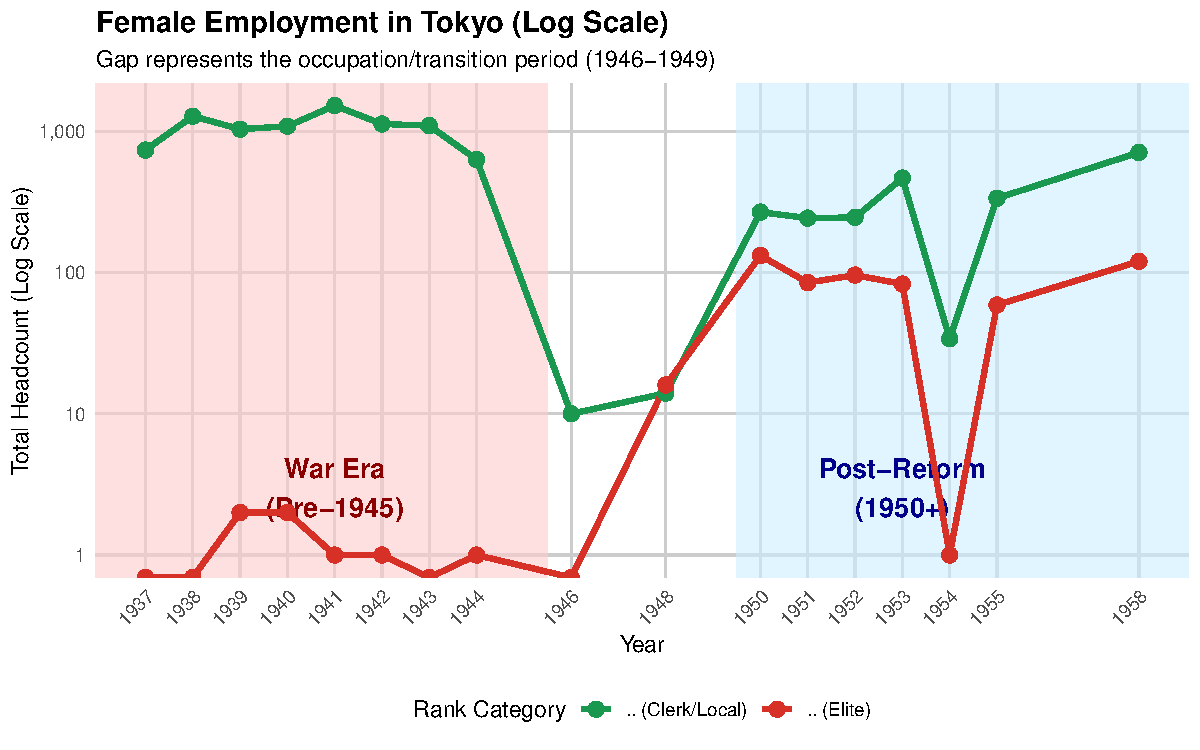
\includegraphics[width=\linewidth]{Institutional Background/Tokyo_Female_Employment_Beamer.pdf}
        \label{fig:placeholder}
    \end{figure}
\end{frame}

\begin{frame}{Research Question}
    \begin{itemize}
        \item Does prior experience shape organizational differences in response to the removal of hiring restrictions?
    \end{itemize}
\end{frame}

\begin{frame}
\frametitle{Specification: Female Assignment to \textit{Kanri} Positions After 1950 Reform}

\vspace{-0.3em}

\textbf{Second Stage:}
\begin{equation*}
Y_{j,1950} = \beta_1 \, \widehat{FemExp}_{j}^{\text{war}} + \beta_2 \, NewHires_{j,1948\text{-}50} + \gamma \, X_j + \alpha_d + \delta_j^{\text{vac}} + \varepsilon_j
\end{equation*}

\textbf{First Stage:}
\begin{equation*}
FemExp_{j}^{\text{war}} = \pi \, Z_j^{\text{draft}} + \phi \, NewHires_{j,1948\text{-}50} + \tilde{\gamma} \, X_j + \tilde{\alpha}_d + \tilde{\delta}_j^{\text{vac}} + \nu_j
\end{equation*}

\vspace{0.3em}
\small
\begin{tabular}{@{}l@{\;}l}
$Y_{j,1950}$ & = female share (or indicator) among \textit{kanri} in office $j$ in 1950 \\[3pt]
$FemExp_{j}^{\text{war}}$ & = avg.\ female share among wartime incumbents still in office $j$ post-war \\[3pt]
$NewHires_{j,1948\text{-}50}$ & = composition of post-war new hires in office $j$ (number, female share) \\[3pt]
$Z_j^{\text{draft}}$ & = share of office $j$'s pre-war workers drafted during 1937--44 (instrument) \\[3pt]
$\alpha_d$ & = department/division fixed effects (compare offices providing similar services) \\[3pt]
$\delta_j^{\text{vac}}$ & = vacancy control: indicator for whether the \textit{kanri} in office $j$ in 1948 separated \\[3pt]
$X_j$ & = pre-war office size, occupation mix, share of higher-class employees
\end{tabular}
\end{frame}

\end{document}